\chapter{Présentation de la solution sélectionnée}

\section{Vue d'ensemble}

La solution retenue est un module de test unitaire conçu pour mesurer automatiquement la réserve de marche d'un mouvement horloger.
Le prototype complet est visible à la figure~\ref{fig:vue_ensemble}.

\begin{figure}[H]
    \centering
    \fbox{\parbox{0.85\textwidth}{\centering\vspace{2.5cm}\textit{[Photo : vue d'ensemble du prototype assemblé]}\vspace{2.5cm}}}
    \caption{Vue d'ensemble du module de test assemblé}
    \label{fig:vue_ensemble}
\end{figure}

Le module est articulé autour de quatre sous-systèmes fonctionnels complémentaires :

\begin{enumerate}
    \item Système de fixation~: maintien du mouvement en position stable pendant toute la durée du test.
    \item Système de motorisation~: entraînement contrôlé de la tige de remontoir, avec limitation du couple appliqué sur le mouvement.
    \item Système d'accouplement~: liaison mécanique entre l'arbre moteur et la tige du mouvement, sans transmission d'efforts radiaux.
    \item Système d'acquisition optique~: prise de vue périodique du mouvement permettant de détecter automatiquement son arrêt.
\end{enumerate}

L'ensemble est piloté depuis un ordinateur via un script Python, sans microcontrôleur intermédiaire.

\section{Système de fixation}

Le mouvement est maintenu en place par un porte-mouvement industriel (figure~\ref{fig:fixation_proto}).
Il accueille l'ensemble des calibres définis dans le cahier des charges et permet un montage en moins de deux minutes, sans outillage et surtout sans endommager les composants du mouvement.

\begin{figure}[H]
    \centering
    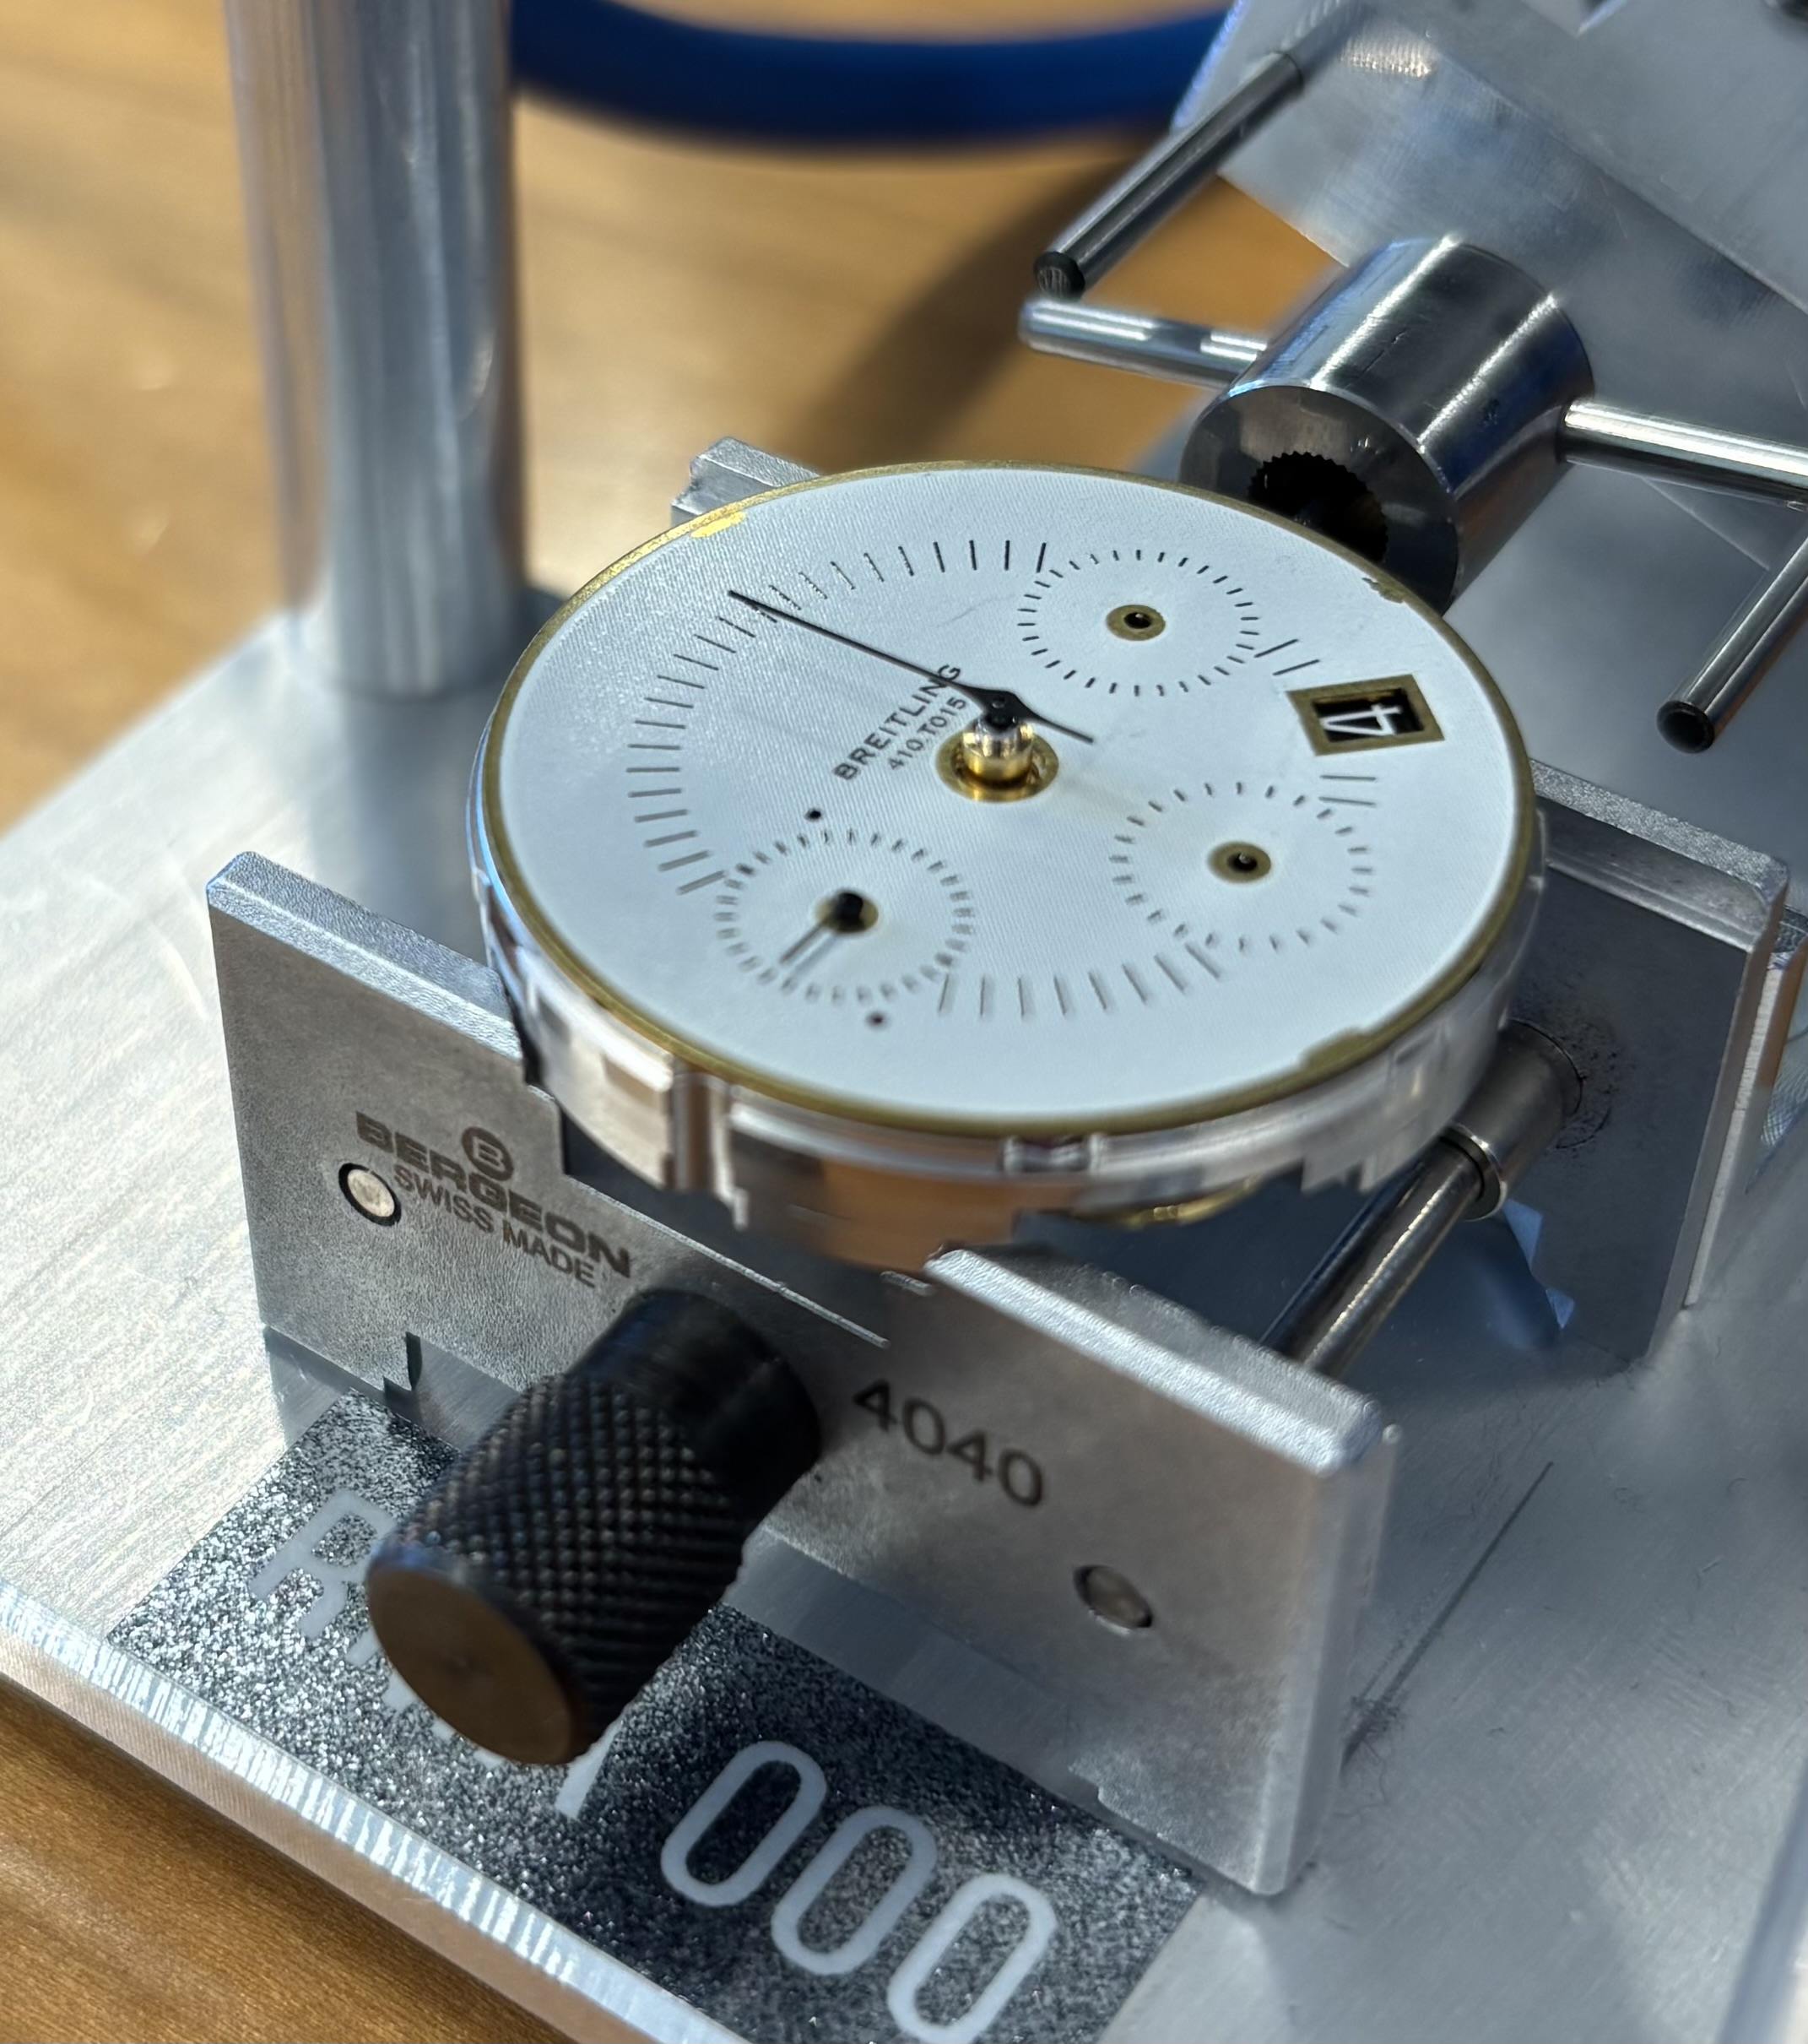
\includegraphics[width=0.65\textwidth]{assets/figures/Solution/Systeme de fixation du mouvement.jpg}
    \caption{Porte-mouvement avec un calibre en position de test}
    \label{fig:fixation_proto}
\end{figure}

Cette solution est déjà utilisée régulièrement et a même été recommandé par Breitling. 
Par conséquent, cette solution de fixation semble idéal pour le projet.

\section{Système de motorisation}

Un moteur pas à pas de format NEMA 11 entraîne la tige de remontoir (figure~\ref{fig:moteur_proto}).
Ce type de moteur a été retenu pour sa capacité à contrôler précisément la position angulaire et à maintenir une position bloquée sans alimentation — deux propriétés indispensables pour les phases de remontage et d'attente du test.

\begin{figure}[H]
    \centering
    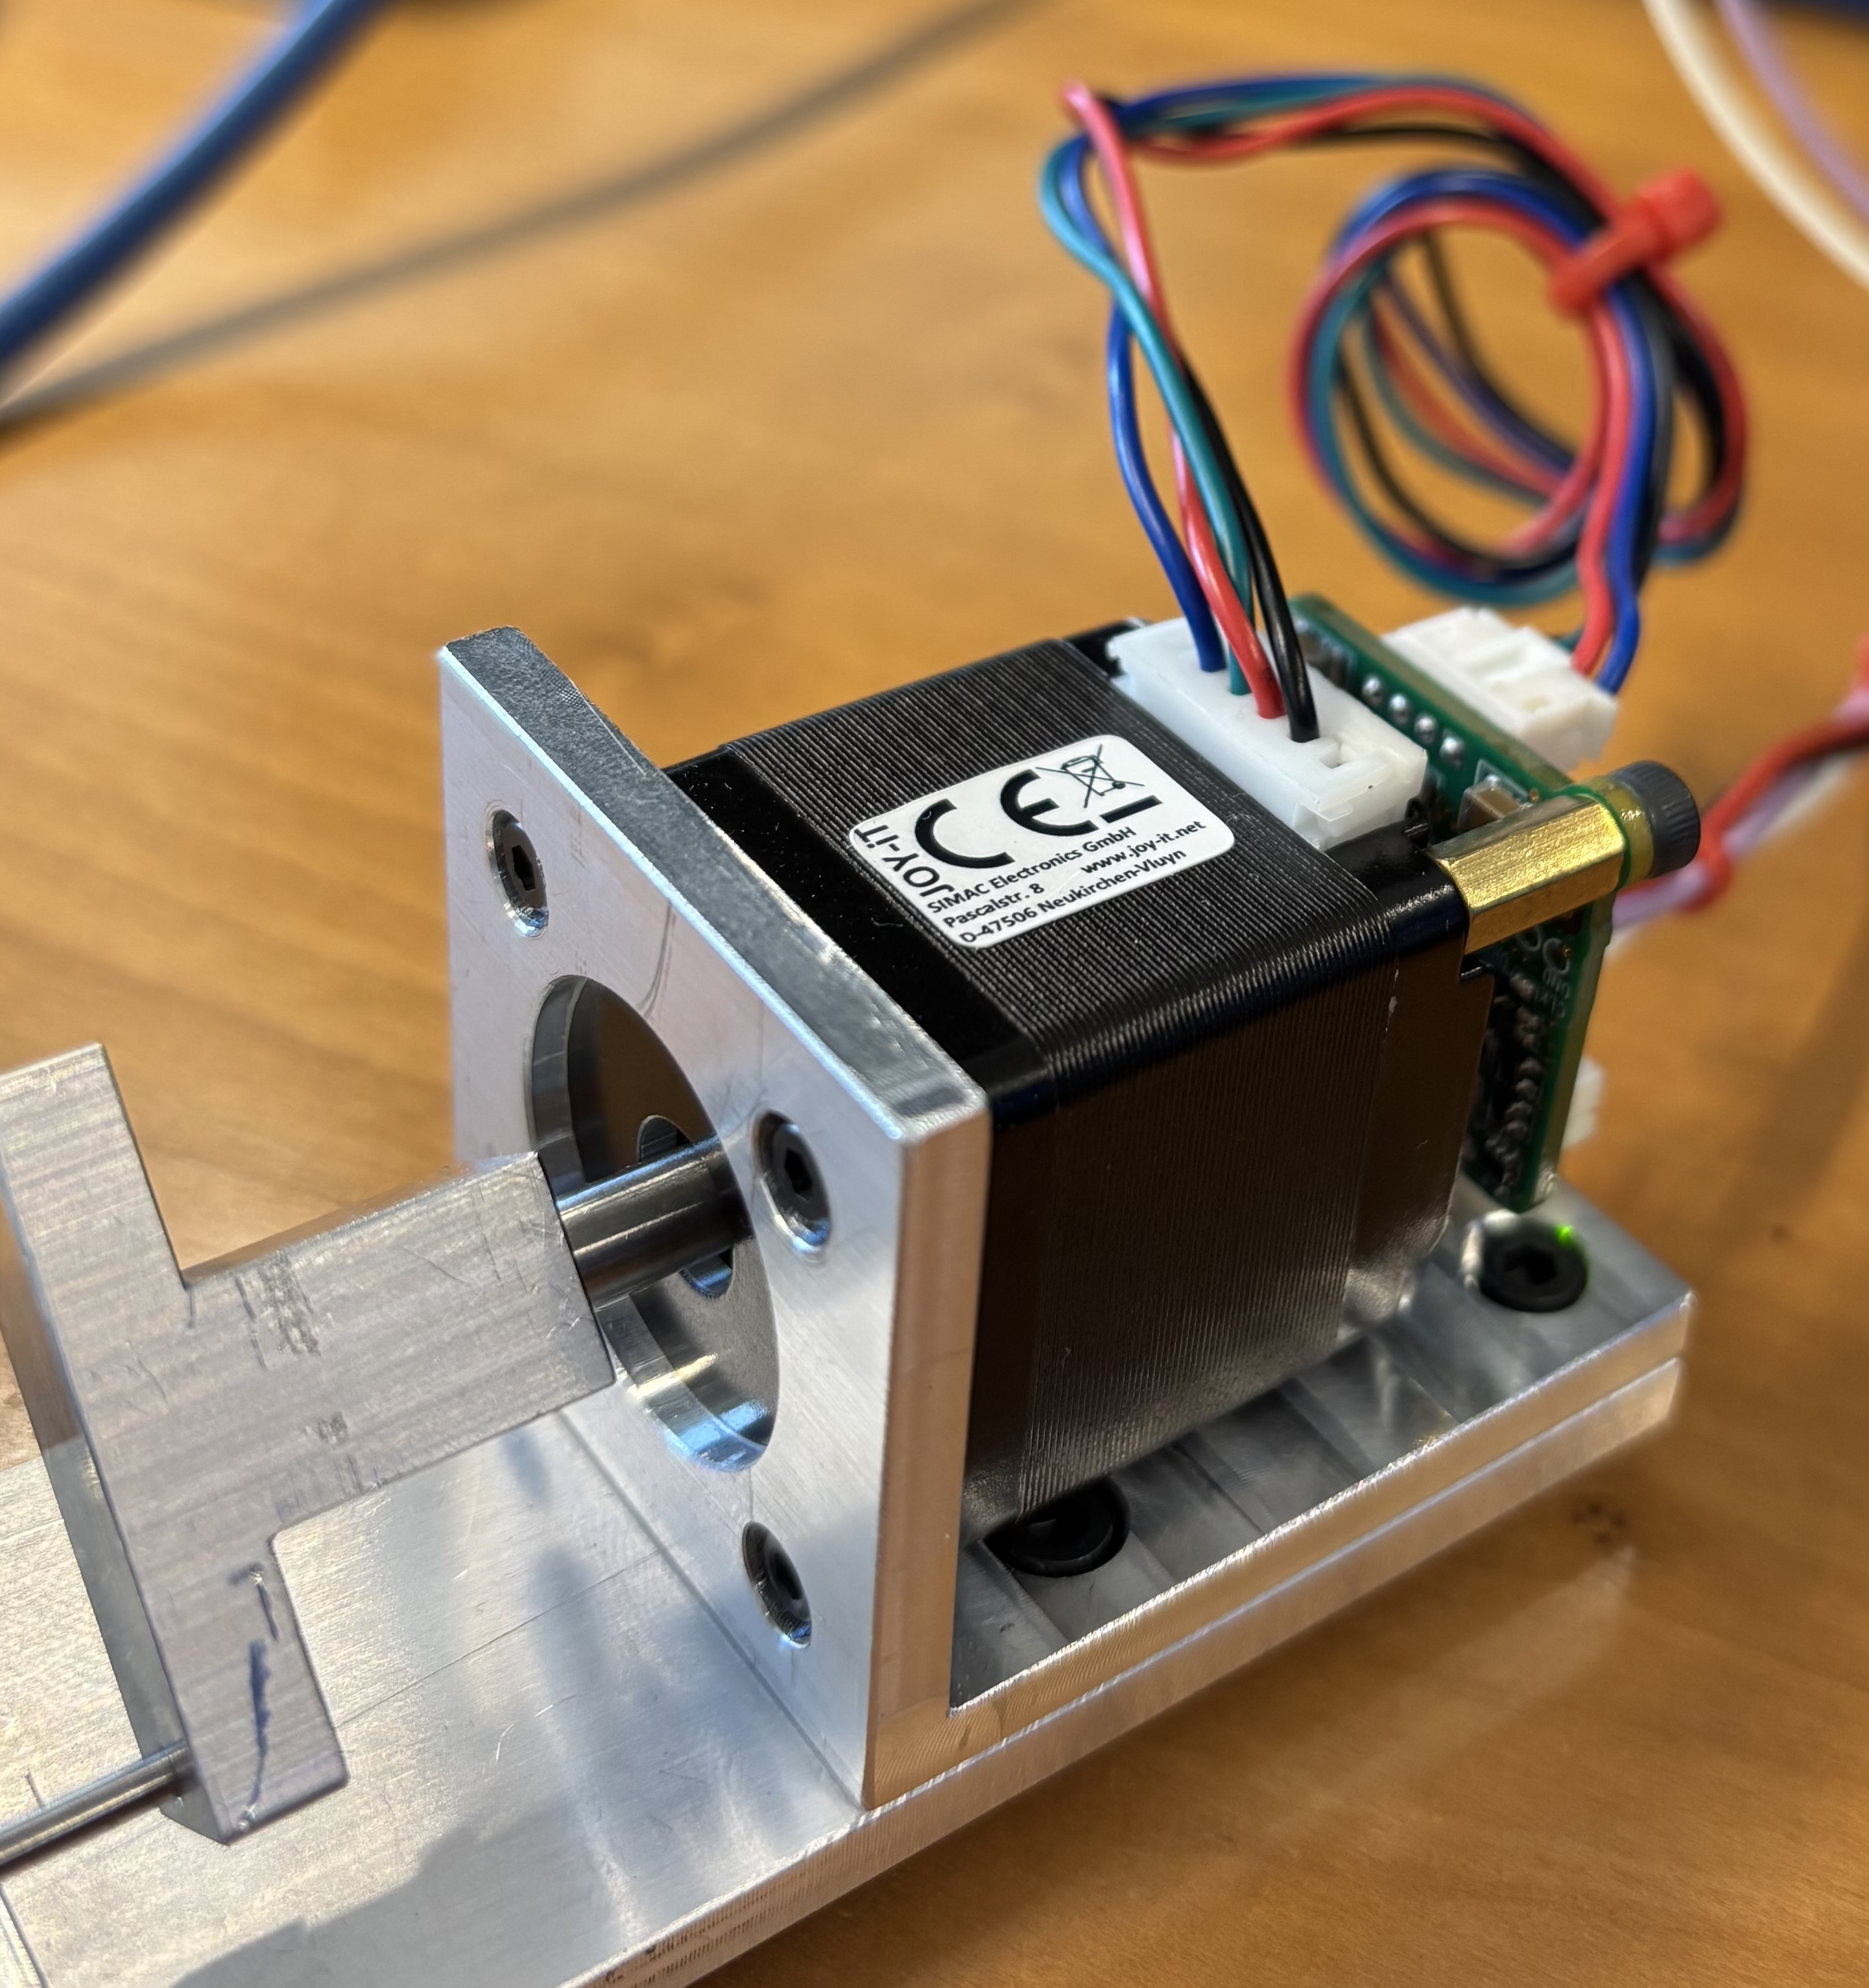
\includegraphics[width=0.65\textwidth]{assets/figures/Solution/Montage du moteur pas à pas.jpg}
    \caption{Moteur pas à pas NEMA 11 monté sur la structure}
    \label{fig:moteur_proto}
\end{figure}

Le driver électronique, monté directement à l'arrière du moteur, est raccordé à l'ordinateur via une liaison RS485.
Il assure la limitation de courant, et donc du couple transmis à la tige, garantissant que le mouvement n'est jamais sollicité au-delà des limites définies dans le cahier des charges.

\section{Système d'accouplement}

La liaison entre l'arbre moteur et la tige de remontoir est réalisée par un accouplement de type fourche–T (figure~\ref{fig:accouplement_proto}).
Une pièce en forme de T solidaire de l'arbre s'engage dans une fourche à deux ergots montée sur la tige.

\begin{figure}[H]
    \centering
    \fbox{\parbox{0.65\textwidth}{\centering\vspace{2.5cm}\textit{[Photo : accouplement fourche–T assemblé]}\vspace{2.5cm}}}
    \caption{Accouplement fourche–T assemblé entre le moteur et la tige du mouvement}
    \label{fig:accouplement_proto}
\end{figure}

Ce principe transmet le couple de rotation tout en découplant les axes radiaux : les charges radiales et les légères erreurs d'alignement entre les deux axes ne sont pas transmises à la tige, protégeant ainsi le mouvement.

\section{Système d'acquisition optique}

Une caméra industrielle est fixée au-dessus du mouvement à une distance de travail de 300 mm (figure~\ref{fig:camera_proto}).
Toutes les 15 minutes, une photo est prise.
Un algorithme de traitement d'image compare chaque nouvelle image à la précédente~: dès que les aiguilles n'ont plus bougé, l'arrêt du mouvement est détecté et la réserve de marche est calculée.

\begin{figure}[H]
    \centering
    \fbox{\parbox{0.65\textwidth}{\centering\vspace{2.5cm}\textit{[Photo : caméra et ring light au-dessus du mouvement]}\vspace{2.5cm}}}
    \caption{Caméra et ring light positionnées au-dessus du mouvement en test}
    \label{fig:camera_proto}
\end{figure}

Une ring light coaxiale à l'objectif, combinée à un filtre polarisant croisé, supprime les reflets spéculaires sur les composants métalliques du mouvement.
Cet éclairage garantit une qualité d'image constante indépendante des conditions lumineuses de l'atelier, conformément à la contrainte FC8 du cahier des charges.
